\documentclass [a4paper,11pt]{article}
\usepackage{amssymb}
\usepackage{amsthm}
\usepackage[intlimits]{amsmath}
\usepackage[polish]{babel}
\usepackage[utf8]{inputenc}
\usepackage[T1]{fontenc}
\frenchspacing
\usepackage{indentfirst}
\usepackage{graphicx}
\usepackage{subfig}
\usepackage{mathptmx}
\usepackage{geometry}
\usepackage{wrapfig}
\usepackage{enumitem}

\title{Opracowanie danych pomiarowych}
\author{Pęcak Tomasz, Bielech Maciej}
\begin{document}
	
	\renewcommand*{\figurename}{Tabela} 
	\newgeometry{tmargin=2cm, bmargin=2cm, lmargin=2cm, rmargin=2cm}
	
	\linespread{1.5}
	\selectfont

	\begin{table}[]
		\centering
		\begin{tabular}{lllllll}
			\cline{1-6}
			\multicolumn{1}{|c|}{\begin{tabular}[c]{@{}c@{}}EAiIB\\ Informatyka\end{tabular}} & \multicolumn{2}{l|}{\begin{tabular}[c]{@{}l@{}}Pęcak Tomasz\\ Bielech Maciej\end{tabular}} & \multicolumn{1}{c|}{\begin{tabular}[c]{@{}c@{}}Rok\\ II\end{tabular}} & \multicolumn{1}{c|}{\begin{tabular}[c]{@{}c@{}}Grupa\\ 3a\end{tabular}} & \multicolumn{1}{c|}{\begin{tabular}[c]{@{}c@{}}Zespół\\ II\end{tabular}} &  \\ \cline{1-6}
			\multicolumn{1}{|c|}{\begin{tabular}[c]{@{}c@{}}Pracownia\\ FIZYCZNA\\ WFiIS AGH\end{tabular}} & \multicolumn{4}{l|}{\begin{tabular}[c]{@{}l@{}}Temat:\\ \textbf{Opracowanie danych pomiarowych} \end{tabular}} & 
			\multicolumn{1}{l|}{\begin{tabular}[c]{@{}l@{}}nr ćwiczenia:\\ 0\end{tabular}} &  \\ \cline{1-6}
			\multicolumn{1}{|l|}{\begin{tabular}[c]{@{}c@{}}Data wykonania:\\ 14.10.2017\end{tabular}} & \multicolumn{1}{c|}{\begin{tabular}[c]{@{}c@{}}Data oddania:\\ 18.10.2017\end{tabular}} & \multicolumn{1}{l|}{\begin{tabular}[c]{@{}l@{}}Zwrot do poprawki:\\ \phantom{data poprawki}\end{tabular}} & \multicolumn{1}{l|}{\begin{tabular}[c]{@{}l@{}}Data oddania:\\  \phantom{data oddania}\end{tabular}} & \multicolumn{1}{l|}{\begin{tabular}[c]{@{}l@{}}Data zaliczenia:\\  \phantom{data zaliczenia}\end{tabular}} & \multicolumn{1}{l|}{\begin{tabular}[c]{@{}l@{}}OCENA:\\ \phantom{ocena}\end{tabular}} &  \\ \cline{1-6} 
		\end{tabular}
	\end{table}
	 \hspace{5mm}

	\section{Wstęp}\label{wstep}
	Celem ćwiczenia było wyznaczenie przyspieszenia ziemskiego przy użyciu wahadła matematycznego na dwa różne sposoby oraz zapoznanie się z metodami opracowania danych pomiarowych.
	
	 Wahadło matematyczne jest przykładem oscylatora harmoniczego.
	Składa się z ciała o masie punktowej zawieszonego na nierozciągliwej nici, np. ciężarek na lince. Po wytrąceniu cieżarka z równowagi zaczyna on drgać pod wpływem siły grawitacji. 
	
	Pomimo, że wahadło matematyczne jest stosunkowo prostym narzędziem, korzystając z niego możemy wyznaczyć przyspieszenie ziemskie na kilka sposobów. W naszym ćwiczeniu skorzystaliśmy z dwóch takich metod. W obu z nich  wykorzystaliśmy wzór na okres wahadła: 
	\begin{equation}
	\label{eq:wokres} 
	T= 2 \pi \sqrt{\frac{l}{g}} \text{ .}
	\end{equation}
	
	Jest on słuszny tylko wtedy, kiedy wartość sinusa jest równa w przybliżeniu wartości kąta wyrażonego w~radianach.
	Przyjeliśmy, że taka sytuacja zachodzi dla kątów nie większych od $3^\circ$.
	
	Przekształcając wzór (\ref{eq:wokres}) możemy wyznaczyć wartość przyspieszenia ziemskiego:
	\begin{equation}
	\label{eq:wprzysp} 
	g= \frac{4 \pi^2 l}{T^2} \text{ .}
	\end{equation}
	
	W celu opracowania wyników skorzystaliśmy z następujących metod:
	\begin{itemize}
		\item Analiza błędów.
		\item Ocena niepewności typu A.
		
		Ocenę niepewności typu A stosujemy, gdy pomiary są obarczone błędem przypadkowym. Najczęściej ta niepewność jest wykorzystywana dla analizy wielkrotnej obserwacji tego samego doświadczenia. Do obliczenia przybliżeń wykorzystujemy estymatory: odchylenia standardowego, który jest miarą rozrzutu wyników pomiarów:
		\begin{equation}
		\label{eq:estymator}
		s_x = \sqrt{\frac{\sum (x_i -x_0)^2}{n-1}}
		\end{equation}
		oraz estymator odchylenia standardowego średniej, który przyjmujemy jako wyznaczaną niepewność pomiaru:
		\begin{equation}
			\label{eq:estymatorsredniej}
			s_{x_0}=\frac{s_x}{\sqrt{n}} \text{.}
		\end{equation}
		Przy obliczaniu wyżej wymienionych estymatorów, za wartość dokładną przyjmuje się średnią arytmetyczną pomiarów:
		\begin{equation}
		\label{eq:wstepsrednia}
		x \equiv x_0 = \frac{1}{n}\sum x_i
		\end{equation}
		
		\item Ocena niepewności typu B.
		
		Ocene tę wyliczamy, gdy niemożliwe jest wyliczenie oceny niepewności typu A. Użyliśmy jej w drugiej części ćwiczenia, gdyż do dyspozycji mieliśmy jedynie jeden wynik pomiaru dla danej długości wahadła. Do jej określenia posłużyliśmy się znajomością niedokładności przyrządów pomiarowych.
		
		\item Prawo przenoszenia niepewności.
		
		Pomiar przyspieszenia był obarczony błędem pomiaru długości wahadła i pomiaru czasu dwudziestu okresów, dlatego też skorzystaliśmy z prawa przenoszenia niepewności:
		\begin{itemize}
			\item Policzenie niepewności złożonej jako:
			\begin{equation}
			\label{eq:wstepprzenoszenie1}
			u_c(y) = \sqrt{\sum_k \left[ \frac{\partial y}{\partial x_k}u(x_k) \right]^2}\text{,}
			\end{equation}
			\item Wyznaczenie niepewności względnej: 
			\begin{equation}
			\label{eq:wstepprzenoszenie2}
			\frac{u_c(y)}{y} = \frac{1}{y}\sqrt{\sum_k \left[ \frac{\partial y}{\partial x_k}u(x_k) \right]^2} = \sqrt{\sum_k \left[ \left( \frac{\partial y}{\partial x_k}\cdot \frac{x_k}{y} \right)\cdot \frac{u(x_k)}{x_k} \right]^2}\text{,}
			\end{equation}
		\end{itemize}
		
		\item Obliczanie niepewności rozszerzonej.
		
		Aby policzyć niepewność rozszerzoną mnożymy wartość niepewności złożonej przez współczynnik rozszerzenia $k$, przyjmując, że jest równy 2:
		\begin{equation}
		\label{eq:wsteprozszerzona}
		U(y) = k \cdot u_c(y)
		\end{equation}
		
		\item Wykonywanie tabel/wykresów.
		\item Regresja liniowa.
		
		W drugiej części ćwiczenia wykorzystaliśmy metodę regresji liniowej. Metoda ta jest przybliżaniem wykresu wykonanego podczas przenoszenia pomiarów do funkcji liniowej. Mogliśmy tak postąpić, gdyż wyniki powinny przyrastać liniowo. Wykres regresji liniowej został wykonany przy użyciu programu Microsoft Excel. 
		
	\end{itemize}
	\newpage
	\section{Wykonanie ćwiczenia}
	Ćwiczenie było podzielone na dwie części. Każda część to jedna z metod (wspomianych we wstępie) wyznaczania grawitacji za pomocą wahadła matematycznego.
	\begin{itemize}
		\item Część I - Pomiary okresu dla ustalonej długości wahadła.
		
		W pierwszym kroku dokonaliśmy pomiaru długości wahadła przy użyciu linijki milimetrowej z~dokładnością 1 mm. Korzystając ze zmierzonej długości obliczyliśmy przybliżoną amplitudę drgań.
		\begin{equation}
			\label{eq:amplituda} 
			A \approx l \frac{\pi}{60} 
		\end{equation}
		$$ A \approx  18 \text{ mm}$$
		Następnie dziesięciokrotnie wykonaliśmy pomiar czasu dwudziestu okresów dbając o odpowiednie początkowe wychylenie wahadła (nie większe niż wyliczona amplituda).
		
		Otrzymane wyniki nanieśliśmy do tabeli (\ref{fig:czescpierwsza}).
		
		\begin{figure}[!h]
			\centering
			\caption{Pomiary - część pierwsza}
			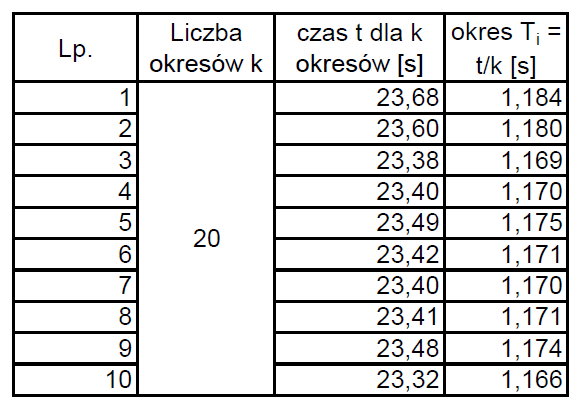
\includegraphics[width=0.5\textwidth]{wykres1}
			\label{fig:czescpierwsza}
		\end{figure}
		
		\item Część II - Pomiary zależności okresu drgań od długości wahadła.
		
		W tej części wyznaczaliśmy czas dwudziestu okresów dla różnych długości wahadła w celu znalezienia ich zależności. Pomiary rozpoczeliśmy od najmniejszej długości nici, dla której amplituda nie była zbyt mała i~wyznaczanie okresów było możliwe. Po każdym pomiarze zwiększaliśmy długość wahadła poprzez odwijanie nici ze statywu. Długość nici nie pozwoliła na wykonanie więcej niż 10 pomiarów.
		
		Otrzymane wyniki nanieśliśmy do tabeli (\ref{fig:czescdruga}).
		
		\begin{figure}[!h]
			\centering
			\caption{Pomiary - część druga}
			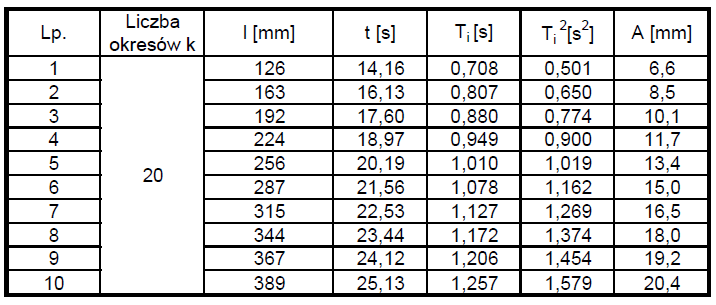
\includegraphics[width=0.7\textwidth]{tab2}
			\label{fig:czescdruga}
		\end{figure}
	\newpage
	\end{itemize}
	
	\section{Opracowanie danych pomiarowych}
	\subsection{Część pierwsza}\label{cz1}
	\begin{enumerate}[label=\alph*)]
		\item Analiza błędów.
		
		Nie stwierdzamy błędu grubego, gdyż wartości skrajne nie odbiegają zbytnio od średniej arytmetycznej wszystkich wyników:
		\begin{equation}
		\label{eq:srednia}
			T_{\text{0}}  = \frac{1}{n} \sum_{i=1}^{n} T_i \approx 1,173\text{ s,}
		\end{equation}
		gdzie $n$ to ilość wykonywanych powtórzeń pomiaru czasu.
		
		\item Ocena niepewności pomiaru czasu.
		
		Pomiary były wykonywane dziesięciokrotnie, dlatego wykorzystaliśmy obliczanie niepewności typu A:
		
		\begin{equation}
		\label{eq:odchylenie1}
			s(T_0) = \sqrt{\frac{\sum_{}^{}(T_i-T_0)^2}{n - 1}} = 0,054\text{ s,}
		\end{equation}
		
		\begin{equation}
		\label{eq:odchylenie2}
			u(T_0) = \frac{s(T_0)}{\sqrt{n}} = 0,0017\text{ s.}
		\end{equation}
		
		gdzie (\ref{eq:odchylenie1}) to estymator odchylenia standardowego, a (\ref{eq:odchylenie2}) to estymator odchylenia standardowego średniej.
		
		\item Ocena niepewności pomiaru długości wahadła.
			
			Długość wahadła zmierzyliśmy linijką milimetrową uzyskując wartość l = 344 mm. Przyjmujemy niepewność pomiaru typu B równą: $u(l) = 2 \text{ mm}$. Ocena ta bierze pod uwagę trudność dobrego przyłożenia linijki do odcinka: środek kuli – punkt zawieszenia wahadła.

		
		\item Prawo przenoszenia niepewności.
		
		Przyspieszenie ziemskie obliczamy jako:
		\begin{equation}
		\label{eq:przyspieszenie}
			g=\frac{4\pi^2l}{T_0^2} \approx 9,872 \text{ }\mathrm{\frac{m}{s^2}.}
		\end{equation}
		
		Stosując prawo przenoszenia niepewności, obliczamy niepewność złożoną pomiaru przyspieszenia:
		\begin{equation}
		\label{eq:niepewnosc}
			u_c(g) = \sqrt{ \left[ \frac{4\pi^2}{T_0^2}u(l) \right]^2 + \left[ -\frac{8\pi^2l}{T_0^3}u(T_0) \right]^2} = 0,064 \text{ }\mathrm{\frac{m}{s^2}}
		\end{equation}
		oraz niepewność względną złożoną:
		\begin{equation}
		\label{eq:niepewnoscwzgl}
		\frac{u_c(g)}{g} \approx  0,7 \%\text{.}
		\end{equation}
		
		\item Obliczanie niepewności rozszerzonej.
		
		Różnica pomiedzy obliczoną wartością przyspieszenia, a wartością tabelaryczną wynosi:
		\begin{equation}
		\label{eq:roznica}
			|g - g_0| = \left|9,872 \text{ }\mathrm{\frac{m}{s^2}} - 9,811 \text{ }\mathrm{\frac{m}{s^2}}\right| = 0,061 \text{ }\mathrm{\frac{m}{s^2}}.
		\end{equation}
		Obliczamy niepewność rozszerzoną wyniku:
		\begin{equation}
		\label{eq:rozszerzona}
			U(g) = ku_c(g) = 2 \cdot 0,064 \text{ }\mathrm{\frac{m}{s^2}} = 0,128 \text{ }\mathrm{\frac{m}{s^2}}\text{,}
		\end{equation}
		gdzie k to współczynnik rozszerzenia równy 2.
		
		\item Zastosowanie niepewności rozszerzonej do oceny zgodności z wartością dokładną.
		
		Niepewność rozszerzona wyniku jest większa od modułu różnicy pomiędzy obliczoną wartością przyspieszenia, a wartością tabelaryczną. Uznajemy więc, że policzone przyspieszenie jest zgodne z wartością tabelaryczną w zakresie wyznaczonej niepewności.
	\end{enumerate}
		\subsection{Część druga}
	\begin{enumerate}[label=\alph*)]
		\item Wykres obrazujący wyniki przebiegu części drugiej doświadczenia.
		\renewcommand*{\figurename}{Wykres} 
		\setcounter{figure}{0}
		\begin{figure}[!h]
			\centering
			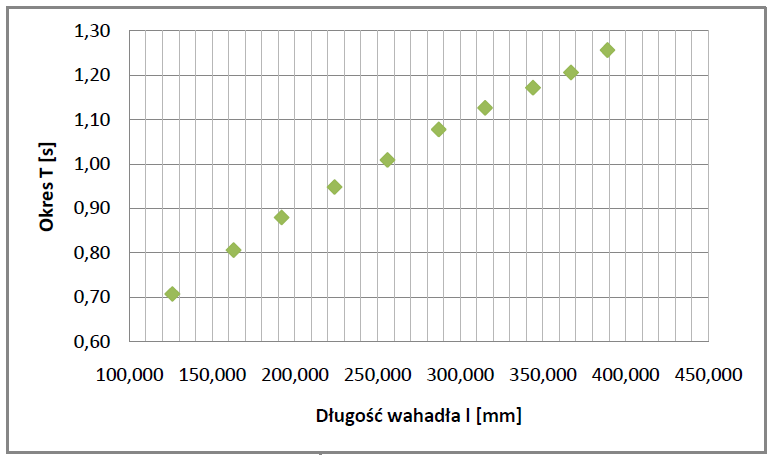
\includegraphics[width=0.8\textwidth]{wyk1}
			\caption{Wykres zależności okresu od długości wahadła}
			\label{fig:w1}
		\end{figure}
	
		Wykres (\ref{fig:w1}) jest wykresem funkcji typu $f(x)=\sqrt{x}$, który jest trudny w analizie, dlatego w celu ułatwienia analizy danych stosujemy linearyzację.
		Podnosimy obie strony wzoru (\ref{eq:wokres}) do kwadratu: 
		\begin{equation}
		\label{eq:kokres} 
		T^2= \frac{4 \pi^2}{g}l \text{ .}
		\end{equation}
		\item Wykres regresji liniowej.
		\begin{figure}[!h]
			\centering
			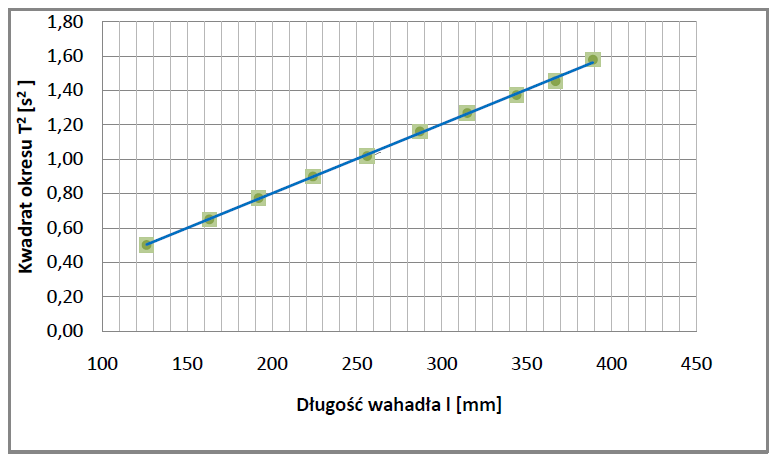
\includegraphics[width=0.9\textwidth]{wykr1}
			\caption{Wykres zależności kwadratu okresu od długości wahadła}
			\label{fig:wykr1}
		\end{figure}
		
		\item Obliczanie niepewności rozszerzonej.
		
		Wykorzystując regresję liniową, obliczamy wartość współczynnika $a$ prostej i  jej dokładność $u(a)$:
		\begin{align}
		a = 4,03 \text{ }\mathrm{\frac{s^2}{m}},\label{a} \\
		u(a) = 0,04 \text{ }\mathrm{\frac{s^2}{m}},
		\end{align}
		
		Stosując prawo przenoszenia niepewności dla funkcji $g = \frac{4\pi^2}{a}$, wyliczamy niepewność złożoną (\ref{eq:niepewnosc2}) i~rozszerzoną (\ref{eq:rozszerzona2}) pomiaru przyspieszenia:
		\begin{equation}
		\label{eq:niepewnosc2}
		u_c(g) = 4\pi^2a^{-2} \cdot u(a) \approx 0,098 \text{ }\mathrm{\frac{m}{s^2}},
		\end{equation}
		\begin{equation}
		\label{eq:rozszerzona2}
		U(g) = k\cdot u_c(g) = 2 \cdot 0,098 \text{ }\mathrm{\frac{m}{s^2}} = 0,196 \text{ }\mathrm{\frac{m}{s^2}}
		\end{equation}
		oraz niepewność względną złożoną:
		\begin{equation}
		\label{eq:niepewnoscwzgl2}
		\frac{u_c(g)}{g} \approx  0,1 \%\text{.}
		\end{equation}
	\end{enumerate}

	\section{Podsumowanie}
	\begin{center}
	\begin{tabular}{|c|c|c|c|c|}
		\hline Opis wielkości & $g \left[ \frac{m}{s^2} \right]$ & $u_c(g) \left[ \frac{m}{s^2} \right]$ & $U(g) \left[ \frac{m}{s^2} \right]$ & $ \frac{u_c(g)}{g} $\\
		\hline Pomiary przy stałej długości wahadła  & 9,872 & 0,064  & 0,128 & 0,7 \% \\ 
		\hline Pomiary przy zmiennej długości wahadła & 9,796  & 0,098  & 0,196 &  1 \%\\ 
		\hline Wartość tablicowa & 9,811  & -  & - & - \\ 
		\hline 
	\end{tabular} 
	\end{center}
	\hspace{1em}
	\begin{itemize}
		\item Pomimo swojej prostoty wahadło matematyczne jest dosyć dokładnym narzędziem do wyznaczania przyspieszenia ziemskiego. 
		
		\item W obu metodach wyniki są zbliżone do wartości tablicowej, a niepewności niewielkie, co sugeruje, że pomiary zostały przeprowadzone poprawnie.
		
		\item Zestawiając obie metody obliczenia przyspieszenia ziemskiego, dokładniejszą okazała się metoda pierwsza (przy stałej długości wahadła). Sposób drugi, mimo wyniku bardziej zbliżonego do wartości tablicowej, ma większą względną niepewność pomiaru.
	\end{itemize}

\end{document}